\documentclass{report}
\usepackage[a4paper, right=2.5cm, left=2.5cm, top=2cm, bottom=2cm]{geometry}
\usepackage[utf8]{inputenc}
\usepackage{amsmath, amsfonts, amssymb, systeme}
\usepackage{stmaryrd}
\usepackage{graphicx}
\usepackage[round]{natbib}
\usepackage{hyperref}
\usepackage{float}
\usepackage{cleveref}
\usepackage{mathrsfs}
\usepackage{todonotes}
\usepackage{nicefrac}

\hypersetup{
    colorlinks=true,
    linkcolor=blue,
    filecolor=magenta,      
    urlcolor=cyan,
    citecolor=blue,
    pdftitle={AS Projet ResNet},
    % pdfpagemode=FullScreen,
}
\urlstyle{same} %\href{url}{Text}

\newtheorem{theorem}{Théorème}
\newtheorem{proof}{Preuve}
\newtheorem{proposition}{Proposition}
\newtheorem{assumption}{Hypothèse}
\newtheorem{definition}{Définition}
\newtheorem{cor}{Corollaire}
\newtheorem{lem}{Lemme}
\newtheorem{note}{Note}
    
\title{Projet d'appentissage statistique\\Facteur de régulation des ResNets profonds}
\author{SHEN Pingya, VIN Charles}
\date{\today}

\begin{document}

\maketitle
\tableofcontents
\chapter{Introduction}
Avant l'introduction de ResNet en 2015 par \citeauthor{resnet}, l'architecture GoogLeNet était le dernier gagnant des challenges de vision par ordinateur. Cette architecture avait été développée pour pallier les problèmes d'apprentissage liés à l'augmentation de la profondeur de VGG, une autre architecture proéminente.

Un réseau plus profond peut offrir de meilleures performances dans certaines conditions, mais il est aussi sujet à des problèmes tels que l'explosion ou l'évanouissement du gradient de la fonction de coût. Durant la rétropropagation, les grandes ou petites valeurs de gradient peuvent s'amplifier à travers les couches du réseau, entraînant un gradient bien plus grand ou plus petit dans les dernières couches par rapport aux premières. Cet effet est multiplicatif et dépend donc de la profondeur du réseau.

Pour un réseau d'une profondeur $L$, on modélise ces états cachés de chaque couche de dimension $d$ par une séquence $(h_k)_{1 \leq k \leq L}$ avec $h_k \in \mathbb{R}^d, \forall 0 \leq k \leq L$. L'explosion du gradient peut être décrite mathématiquement par, avec une forte probabilité, $\| \frac{\partial \mathscr{L}}{\partial h_0} \| \gg \| \frac{\partial \mathscr{L}}{\partial h_L} \|$, où $\mathscr{L}$ représente la loss et $\left\| \cdot \right\|$ la norme euclidienne.

GoogLeNet, bien qu'offrant une légère amélioration des performances par rapport à VGG, était encore relativement complexe et sa profondeur comparable à celle de VGG, passant de 22 à 16 couches. En 2015, Microsoft introduit ResNet, un modèle allant jusqu'à 152 couches et divisant par deux le nombre d'erreurs de GoogLeNet. Son innovation réside dans l'intégration de \textit{skip connections} entre les couches successives, facilitant le passage du gradient au sein du réseau. Mathématiquement, cela donne la relation récurrente suivante pour la séquence $(h_k)_{1 \leq k \leq L}$ :
\[
    h_{k+1} = h_k + f(h_k, \theta_{k+1})
.\]

où $f(\cdot, \theta_{k+1})$ représente les transformations effectuées par la couche $k$ et paramétrées par $\theta_{k+1} \in \mathbb{R}^p$.

Les ResNets sont devenus la base de nombreux modèles d'apprentissage profond de pointe, s'étendant au-delà du traitement d'images pour inclure des domaines tels que le traitement du langage naturel et l'apprentissage par renforcement. L'idée des \textit{skip connections} a inspiré de nombreuses autres architectures et est devenue une pratique courante dans la conception des réseaux neuronaux profonds.

\begin{figure}[htbp]
    \centering
    % \includegraphics[width=.9\textwidth]{figs/}
    \caption{Example d'architecture pour la vision par ordinateur. \textbf{Bas} : VGG-19 (19.6 billion FLOPs). \textbf{Millieu} : un réseau classique (3.6 billion FLOPs). \textbf{Haut} : Un réseau résiduel (3.6 billion FLOPs) avec la présence de \textit{skip connections} dans chaque bloc. Figure extraite de l'article original de ResNet \citep{resnet}}
    \label{fig:resnet}
\end{figure}

Malgré ces avancées, ResNet rencontre toujours des problèmes de gradient durant l'apprentissage. La méthode traditionnelle pour contrer cela est la normalisation des états cachés après chaque couche (\textit{batch normalization}). Cependant, cette approche a un coût computationnel et dépend fortement de la taille du \textit{batch}. Une alternative est d'incorporer un facteur d'échelle $\alpha_L$ devant le terme résiduel, conduisant au modèle suivant :
\begin{equation}\label{resnet_equation}
    h_{k+1} = h_k + \alpha_L f(h_k, \theta_{k+1})
\end{equation}
Le choix de $\alpha_L$ est crucial et dépend naturellement de la profondeur $L$ du réseau. Il assure que la variance du signal reste stable lors de sa propagation à travers les couches. Cependant, il n'existe actuellement ni preuve formelle ni justification mathématique solide pour le choix de ce facteur de régularisation.

Dans ce cours, nous examinerons les fondements mathématiques pour choisir la valeur de $\alpha_L$ en fonction de $L$ et de la distribution initiale des poids, dans le but d'éviter les problèmes d'apprentissage. Deux axes principaux d'étude seront abordés :
\begin{enumerate}
    \item Le facteur $\alpha_L$ à l'initialisation : L'initialisation des paramètres est cruciale pour la phase d'apprentissage d'un modèle et influe même sur ses capacités de généralisation. Une mauvaise initialisation peut entraîner une divergence ou une disparition rapide du gradient, voire un blocage dans l'apprentissage. L'étude du rôle de $\alpha_L$ lors de l'initialisation est donc pertinente. Nous considérerons que, à l'initialisation, les poids de chaque couche $(\theta_k)_{1 \leq k \leq L}$ sont choisis de manière indépendante et identique selon une loi, typiquement gaussienne ou uniforme sur $\mathbb{R}^p$. 
    % \item L'approche continue : Bien que le réseau neuronal soit constitué de nombreuses couches distinctes, l'ensemble du réseau peut être considéré comme une fonction, lorsqu'il y a suffisament de neurones. L'idée centrale des équations différentielles neuronales est de traiter les couches distincts du réseau comme continues, en supposant que chaque couche subit de petits changements. Ainsi, l'entrée de la couche suivante est considérée comme le résultat de l'intégrale de l'entrée de la couche précédente. Cela peut être comparé au mouvement d'un projet, où le déplacement dans la deuxième seconde peut être approximé par la déplacement dans la première seconde plus la vitesse dans la première seconde (multipliée par l'intervalle de temps d'une seconde).
    % Les équations différentielles neuronales ont ouvert une nouvelle direction pour la théorie et la pratique de l’apprentissage profond et ont été appliquées à la classification d’images, aux séries chronologiques et à d’autres domaines. Tous les réseaux d'apprentissage profond avec des connexions résiduelles peuvent être exprimés approximativement par des équations différentielles neuronales
    \item L'approche continue : Dans les réseaux neuronaux composés de nombreuses couches, l'ensemble peut être considéré comme une fonction continue, particulièrement lorsque le nombre de neurones est élevé. Cette méthode envisage le réseau non pas comme une série de couches discrètes, mais plutôt comme un système continu. En adoptant cette vue, chaque couche est perçue comme une évolution marginale de la précédente, similaire à l'idée derrière les connexions résiduelles de ResNet. On peut imaginer que l'entrée de chaque couche suivante résulte de l'intégration des ajustements minimes apportés par la couche précédente, une approche semblable à la modélisation du mouvement en physique, où la position est intégrée sur le temps.\\
    Les EDN représentent une avancée significative dans la théorie et la pratique de l'apprentissage profond, trouvant des applications dans la classification d'images, l'analyse de séries temporelles et d'autres domaines. Il est intéressant de noter que tout réseau de deep learning doté de connexions résiduelles peut être approximativement exprimé par des équations différentielles neuronales.
\end{enumerate}
\chapter{Le facteur $\alpha_L$ à l'initialisation}

Dans cette section, notre objectif est d'examiner comment le facteur de mise à l'échelle $\alpha_L$ affecte la stabilité des ResNets lors de leur initialisation, en supposant que les poids sont des variables aléatoires indépendantes et identiquement distribuées (i.i.d.). Nous analyserons la modélisation, l'initialisation des paramètres et les hypothèses nécessaires à cette démarche.
% Faire un horizon de la partie "related works" en creusant plus loin ? 

\section{Modèle et hypothèses}
\subsection*{Modèle}
Le modèle est basé sur un ensemble de données composé de $n$ paires $(x_i, y_i)_{1 \leq i \leq n}$ avec $x_i \in \mathbb{R}^{n_{\text{in}}}$ comme vecteur d'entrée et $y_i \in \mathbb{R}^{n_{\text{out}}}$ comme vecteur de sortie à prédire (soit en valeurs continues soit en format \textit{one-hot}). Soit $F_\pi(x) \in \mathbb{R}^{n_{\text{out}}}, x \in \mathbb{R}^{n_{\text{in}}}$ la sortie du ResNet définie par 
\begin{align}\label{ResNet_equation}
    h_0 &= Ax, \nonumber\\
    h_{k+1} &= h_k + \alpha_L V_{k+1}g(h_k, \theta_k), \quad 0 \leq k \leq L - 1, \\
    F_{\pi}(x) &= Bh_L, \nonumber
\end{align}
où $\pi = (A, B, (\theta_k)_{k \leq L}, (V_k)_{1 \leq k \leq L})$ sont les paramètres du modèle avec $A \in \mathbb{R}^{d \times n_{\text{in}}}, B \in \mathbb{R}^{n_{\text{out}} \times d}, \theta_k \in \mathbb{R}^p$ et $V_k \in \mathbb{R}^{d \times d}$ pour $k = 1, \ldots, L$. La fonction $g : \mathbb{R}^d \times \mathbb{R}^p \to \mathbb{R}^d$ représente le choix de l'architecture d'un bloc du ResNet. Nous nous intéressons principalement à la suite des états cachés $(h_k)_{0 \leq k \leq L}$ et non aux changements de dimension permis par les matrices $A$ et $B$.
% Un aspect important du modèle \cite{torchvision2016} est que la fonction de couche prend la forme d'une multiplication matrice-vecteur, ce qui sera crucial pour utiliser les résultats de concentration sur des variables aléatoires ??????? Important ????????? 
Finalement, on définit $l: \mathbb{R}^{n_{\text{out}}} \times \mathbb{R}^{n_{\text{out}}} \to \mathbb{R}_+$ comme la fonction de \textit{loss}, différentiable par rapport à son premier paramètre. Cette \textit{loss} peut être une perte quadratique ou une entropie croisée. L'objectif de l'apprentissage est de trouver le paramètre optimal $\pi$ qui minimise le risque empirique $\mathcal{L}(\pi) = \sum_{i=1}^{n} l(F_\pi(x_i), y_i)$ à travers une descente de gradient stochastique ou l'une de ses variantes.

Durant ce cours, nous nous concentrerons particulièrement sur trois architectures classiques de ResNet, présentées dans la \cref{tab:resnet_architectures} ci-dessous. Il pourrait également être intéressant d'envisager un quatrième modèle intégrant plusieurs couches linéaires ou convolutives.

\begin{table}[H]
    \centering
    \begin{tabular}{lll}
        \hline
        \textbf{Nom} & \textbf{Récurrence} & \textbf{Paramètres} \\ \hline
        res-1 & \( h_{k+1} = h_k + \alpha_L V_{k+1}\sigma(h_k) \) & \( \theta_{k+1} = \emptyset \) \\
        res-2 & \( h_{k+1} = h_k + \alpha_L V_{k+1}\sigma(W_{k+1}h_k) \) & \( \theta_{k+1} = W_{k+1} \) \\
        res-3 & \( h_{k+1} = h_k + \alpha_L V_{k+1}\text{ReLU}(W_{k+1}h_k) \) & \( \theta_{k+1} = W_{k+1} \) \\ \hline
    \end{tabular}
    \caption{Exemples d'architectures ResNet considérées dans l'article. Dans les deux premiers cas, la fonction d'activation \( \sigma \) est telle que, pour tout \( x \in \mathbb{R} \), \( a|x| \leq |\sigma(x)| \leq b|x| \), avec \( \frac{1}{\sqrt{2}} \leq a < b \leq 1 \). Dans les deux derniers cas, \( W_{k+1} \in \mathbb{R}^{d \times d} \).}
    \label{tab:resnet_architectures}
\end{table}

\subsection*{Initialisation des paramètres} 
Nous rappelons que $\theta_k \in \mathbb{R}^p$ et $V_k \in \mathbb{R}^{d \times d}$ sont les paramètres des couches cachées de notre modèle pour tout $k \in \llbracket 1, L \rrbracket$. Ces paramètres sont choisis à l'initialisation comme la réalisation de variables aléatoires i.i.d., généralement suivant une distribution uniforme ou gaussienne. Cette initialisation est indépendante de $L$ et donc du modèle représenté par $g$, permettant de considérer plusieurs architectures différentes dans notre étude. Nous examinerons également d'autres approches dépendantes du modèle pour étudier le choix de $\alpha_L$ (par exemple, Yang et Schoenholz, 2017 ou Wang et al., 2022 \cite{torchvision2016}).

\subsection*{Hypothèses}
Pour notre première hypothèse, nous avons besoin de la définition suivante :
\begin{definition}[Variable aléatoire $s^2$ sub-gaussienne]
    En théorie des probabilités, une distribution $s^2$ sub-gaussienne est une distribution de probabilité caractérisée par une décroissance rapide des queues de distribution. Bien qu'il existe de nombreuses définitions et propriétés, nous retiendrons dans ce cours la suivante : soit $X$ une variable aléatoire réelle,
    \[
        \forall \lambda \in \mathbb{R}, \mathbb{E}[\exp(\lambda X)] \leq \exp\left(\frac{\lambda^2 s^2}{2}\right).
    \]
    De manière informelle, les queues d'une distribution sub-gaussienne sont dominées par celles d'une distribution gaussienne, c'est-à-dire qu'elles décroissent au moins aussi rapidement.
\end{definition}

Avec cette définition en tête, passons aux hypothèses. Pour tout $ 1 \leq  k \leq L  $
\begin{assumption}\label{H1}
    Pour un certain $ s \geq 1 $, les entrées de  $ \sqrt{d}V_k $ sont des variables aléatoires symétriques i.i.d., $ s^2 $ sub-gaussiennes, indépendantes de $ d $ et $ L $ et de variance unitaire.
\end{assumption}
\begin{note}
    L'hypothèse \ref{H1} est en pratique satisfaite par toutes les initialisations, en particulier celle par défaut dans les paquets Keras \cite{chollet2015keras} et Torch Vision \cite{torchvision2016}.
    % Cette hypothèse permet de .... dans la preuve ... ?? Tant pis :’(
\end{note}

\begin{assumption}\label{H2}
    Pour un certain $ C > 0 $, indépendant de $ d $ et $ L $, et pour tout $ h \in \mathbb{R}^D  $ 
    \[
        \frac{\left\| h \right\| ^2}{2 } \leq  \mathbb{E }[ \left\|  g(h, \theta _ k ) \right\| ^2 ] \leq \left\| h \right\| ^2
    .\]
    and
    \[
        \mathbb{E } [\left\| g(h, \theta _k)  \right\| ^8 ]\leq C \left\| h  \right\| ^8
    .\]
\end{assumption}
\begin{note}
    La première partie de l'hypothèse \ref{H2} assure que $g(\cdot, \theta_{k+1})$ se comporte approximativement comme une isométrie en moyenne, c'est-à-dire qu'elle préserve les longueurs et les mesures d'angles entre son espace de départ et son espace d'arrivée.

    La deuxième partie de l'hypothèse \ref{H2} vise à limiter les variations excessives dans la norme de $g(h_k, \theta_{k+1})$.
\end{note}

\begin{proposition}[Admis]\label{prop1}
    Soit les modèles \textit{res-1}, \textit{res-2}, \textit{res-3} décrit dans la \Cref{tab:resnet_architectures}, on a \begin{itemize}
        \item [(i)] L'\Cref{H2} est valide pour l'architecture \textit{res-1}
        \item [(ii)] L'\Cref{H2} est valide pour les architectures \textit{res-2} et \textit{res-3} dès lors que les entrées de $ \sqrt{d}W_{k+1}, 0 \leq k \leq L-1 $ sont des variables aléatoire de variance unitaire, i.i.d., symétriques, sub-gaussienne et indépendante de $ d $ et $ L $
    \end{itemize}
\end{proposition}


\begin{lem}[Admis]\label{lem14}
    Considérons un ResNet [\ref{resnet_equation}] tel que les hypothèses \ref{H1} et \ref{H2} soient satisfaites.
    \[
        ((1 + \frac{\alpha _L ^2 }{2 }) ^L - 1) \leq \mathbb{E}( \frac{\left\| h_L - h_0 \right\| ^2 }{\left\| h_0 \right\| ^2}) \leq ((1 + \alpha _L ^2 ) ^L - 1 )
    .\]
\end{lem}
Ce lemme nous servira en particulier dans la preuve de la proposition \ref{prop2}.

\section{Limite probabilistique de la norme des états cachés}

Dans cette section, nous nous intéressons à la quantité $ {\left\| h_L - h_0 \right\|} / {\left\| h_0 \right\|}$. Cette mesure permet d'analyser la valeur des états cachés entre le début et la fin du réseau. Si $\left\| h_L - h_0 \right\| \ll \left\| h_0 \right\|$, cela suggère que le réseau agit presque comme une fonction identité. À l'inverse, un ratio $\left\| h_L - h_0 \right\| \gg \left\| h_0 \right\|$ indique une explosion des valeurs des états cachés. Une situation équilibrée serait représentée par $\left\| h_L - h_0 \right\| \approx \left\| h_0 \right\|$.

Nous appliquerons un raisonnement similaire aux gradients avec la quantité ${\left\| \frac{\partial \mathcal{L}}{\partial h_0} - \frac{\partial \mathcal{L}}{\partial h_L} \right\|} / {\left\| \frac{\partial \mathcal{L}}{\partial h_L} \right\|}$. En raison de la propagation rétroactive du gradient qui commence à partir de la fin du réseau, cette mesure est comparée à la dernière valeur du gradient $\frac{\partial \mathcal{L}}{\partial h_L}$.

Les propositions et corollaires suivants décriront comment le rapport ${\left\| h_L - h_0 \right\|} / {\left\| h_0 \right\|}$ se comporte en fonction de $L\alpha_L$, en établissant différentes bornes supérieures et inférieures.


\begin{proposition}\label{prop2}
    Considérons un ResNet [\ref{resnet_equation}] tel que les hypothèses \ref{H1} et \ref{H2} soient satisfaites.
    Si \( L\alpha_L^2 \leq 1 \), alors, pour tout \( \delta \in (0, 1) \), avec une probabilité d'au moins \( 1 - \delta \),
    \[
        \frac{\|h_L - h_0\|^2}{\|h_0\|^2} \leq \frac{2L\alpha_L^2}{\delta}
    .\]
\end{proposition}
La proposition \ref{prop2} par sa borne supérieur petite indique que le réseau se comporte comme une fonction identité dans le cas où $ L \alpha ^2 _L \ll 1 $.

\begin{proof}[\Cref{prop2}]
    En se basant sur le \cref{lem14}, on a 
    \[
        \mathbb{E}( \frac{\left\| h_L - h_0 \right\| ^2 }{\left\| h_0 \right\| ^2}) \leq ((1 + \alpha _L ^2 ) ^L - 1 )
    .\]
    En se basant sur le lemme \ref{lem14}, considérons le cas où $L \alpha_L^2 \leq 1$ (valeur faible) et $L$ tend vers de grandes valeurs. Dans ce contexte, $(1 + \alpha_L^2)^L$ est une bonne approximation de $\exp(L \alpha_L^2)$ par définition, tout en restant inférieur ou égal à celui-ci en raison de la croissance exponentielle de la fonction $\exp$. En effet, $(1 + \alpha_L^2)^L$ se rapproche de $1 + L \alpha_L^2$ selon la formule du binôme de Newton, et correspond aux premiers termes du développement en série de Taylor de l'exponentielle. Finalement, on a obtiens
    \[
        (1 + \alpha _L ^2)^L -1 \leq \exp (L \alpha _L ^2) - 1
    .\]
    En poursuivant avec le développement de Taylor, nous obtenons une majoration plus précise.
    \[
        (1 + \alpha _L ^2)^L -1 \leq \exp (L \alpha _L ^2) - 1) \leq L \alpha _L ^2 \leq 2 L \alpha _L ^2
    .\]
    Ainsi on obtient 
    \[
        \mathbb{E}( \frac{\left\| h_L - h_0 \right\| ^2 }{\left\| h_0 \right\| ^2}) \leq 2 L \alpha _L ^2
    .\]
    En appliquant l'inégalité de Markov, nous parvenons au résultat souhaité.
\end{proof}



\begin{proposition}[Admise]\label{prop3}
    Considérons un ResNet [\ref{resnet_equation}] tel que les hypothèses \ref{H1} et \ref{H2} soient satisfaites.
    \begin{itemize}
        \item[(i)] Supposons que $ d \geq 64 $ et $ \alpha _L ^2 \leq  \frac{2 }{(\sqrt{C } s^4 + 4 \sqrt{C } + 16 s ^4)d} $. Alors, pour tout $ \delta \in (0, 1) $, avec une probabilité d'au moins $ 1 - \delta $,
        \[
            \frac{\|h_L - h_0\|^2}{\|h_0\|^2} > \exp\left(\frac{3L\alpha_L^2}{8} - \sqrt{\frac{11L\alpha_L^2}{d\delta}}\right) - 1,
        \]
        à condition que
        \[
            2L \exp\left(-\frac{d}{64\alpha_L^2s^2}\right) \leq \frac{\delta}{11}.
        \]
        \item[(ii)] Supposons que $ \alpha_L^2 \leq \frac{1}{\sqrt{C}(d + 128s^4)} $. Alors, pour tout $ \delta \in (0, 1)$, avec une probabilité d'au moins $1 - \delta $,
        \[
            \frac{\|h_L - h_0\|^2}{\|h_0\|^2} < \exp\left(L\alpha_L^2 + \sqrt{\frac{5L\alpha_L^2}{d\delta}}\right) + 1.
        \]
    \end{itemize}
\end{proposition}
La proposition \ref{prop3} aborde les deux cas restants : $L \alpha_L^2 \gg 1$ et $L \alpha_L^2 \approx 1$. Dans la partie \textit{(i)}, la borne inférieure indique une explosion très probable du gradient lorsque $L \alpha_L^2 \gg 1$. La partie \textit{(ii)} traite du cas où $L \alpha_L^2 \approx 1$, avec une borne supérieure qui, en combinaison avec celle de \textit{(i)}, suggère que $h_L$ fluctue autour de $h_0$, étant ainsi borné des deux côtés.

Cette proposition \ref{prop3} peut présenter des hypothèses qui semblent atypiques, mais elles sont en réalité souvent vérifiées dans la majorité des ResNets profonds. En effet, il est courant de trouver des ResNets avec une profondeur $L \geq 100$, pour lesquels on définit généralement $\alpha_L = 1 / L^\beta$ avec $\beta > 0$. De plus, la dimension des états cachés atteint fréquemment des valeurs telles que $d \geq 100$.

Les conséquences des propositions \ref{prop2} et \ref{prop3} vont devenir plus clair en fixant $ \alpha _L = 1/L ^\beta $ comme montré dans le corollaire suivant.
\begin{cor}\label{cor4}
    Considérons un ResNet [\ref{resnet_equation}] tel que les hypothèses \ref{H1} et \ref{H2} soient satisfaites, et soit $ \alpha_L = 1/L^\beta $, avec $ \beta > 0 $.
    \begin{itemize}
        \item[(i)] Si $ \beta > \frac{1}{2} $, alors
        \[
            \frac{\|h_L - h_0\|}{\|h_0\|} \xrightarrow{\mathbb{P}} 0 \text{ lorsque } L \to \infty.
        \]
        \item[(ii)] Si $ \beta < \frac{1}{2}$ et $d \geq 9 $, alors
        \[
            \frac{\|h_L - h_0\|}{\|h_0\|} \xrightarrow{\mathbb{P}} \infty \text{ lorsque } L \to \infty.
        \]
        \item[(iii)] Si $ \beta = \frac{1}{2} $, $ d \geq 64$, $L \geq \left(\frac{1}{2}\sqrt{C}s^4 + 2\sqrt{C} + 8s^4)d + 96\sqrt{C}s^4\right) $, alors, pour tout $ \delta \in (0, 1) $, avec une probabilité d'au moins $ 1 - \delta $,
        \[
            \exp\left(\frac{3}{8} - \sqrt{\frac{22}{d\delta}}\right) - 1 < \frac{\|h_L - h_0\|^2}{\|h_0\|^2} < \exp\left(1 + \sqrt{\frac{10}{d\delta}}\right) + 1,
        \]
        à condition que
        \[
            2L \exp\left(-\frac{Ld}{64s^2}\right) \leq \frac{\delta}{11}.
        \]
    \end{itemize}
\end{cor}
Le corollaire 4 clarifie le comportement de notre dernier état caché $ \left\| h_L \right\|  $ en fonction de $ \beta  $. 
\begin{itemize}
    \item Lorsque $ \beta > 1/2 $, la distance entre $ h_L $ et $ h_0 $ converge vers zéro lorsque $ L $ tend vers l'infinie. Indiquant un réseau aggisant essentiellement comme une fonction identité.
    \item Lorsque $ \beta < 1/2 $, la norme de $ h_L $ explose.
    \item Lorsque $ \beta = 1/2 $, On voit que $ h_L $ fluctue autour de $ h_0 $, indépendament de la longueur du réseau $ L $.
\end{itemize}
On conclu donc que seul fixer $ \beta = 1/2 $ permet d'obtenir une distribution correcte.

Le corollaire 4 précise le comportement de notre dernier état caché $\left\| h_L \right\|$ en fonction de $\beta$.
\begin{itemize}
    \item Lorsque $\beta > 1/2$, la distance entre $h_L$ et $h_0$ tend vers zéro lorsque $L$ augmente indéfiniment. Cela indique que le réseau fonctionne essentiellement comme une fonction identité.
    \item Lorsque $\beta < 1/2$, la norme de $h_L$ tend à l'explosion avec la valeur de $ L $ .
    \item Lorsque $\beta = 1/2$, $h_L$ fluctue autour de $h_0$, indépendamment de la longueur du réseau $L$.
\end{itemize}
En conséquence, fixer $\beta = 1/2$ est la seule manière d'assurer une distribution adéquate des valeurs de $h_L$.


\begin{proof}[\Cref{cor4}]
    L'affirmation ($ i $) est une conséquence de la Proposition \ref{prop2}.
    % Tentative de preuve......
    %%%%%%%%%%%%%%%%%%%%%%%%%%%%%%%%%%%%%%%%%%%%
    % Nous avons $ L \alpha _L ^2 = \frac{L}{L^{2\beta} } = L^{1 - 2 \beta } $, comme $ \beta > 1/2 \Leftrightarrow 1 - 2 \beta < 0 $ nous avons $ L^{1 - 2 \beta } = \frac{1}{L^{2 \beta  -1}} \underset{L\to +\infty}{\longrightarrow} 0 $. Ainsi
    % \begin{align*}
    %     & \frac{\|h_L - h_0\|^2}{\|h_0\|^2} \leq \frac{2L\alpha_L^2}{\delta}.
    %     \overunderset{\mathbb{P}}{L\to +\infty}{\longrightarrow} 0 
    % \end{align*}
    %%%%%%%%%%%%%%%%%%%%%%%%%%%%%%%%%%%%%%%%%%%%
    L'affirmation ($ ii $) est une conséquence de la \Cref{prop3}. En effet, cette dernière est valide les conditions $ d \geq 64 $ et $ \alpha _L \leq \frac{2}{(\sqrt{C} s^4 + 4 \sqrt{C} + 16s^4)d} $. La majoration d'$ \alpha _L $ est automatiquement satisfaite pour $ L $ assez grand. Quant à la contrainte sur $ d $, elle peut être, dans notre cas, relaché à $ d \geq 9 $ en observant la preuve de la \Cref{prop3} non décrite ici.

    Pour prouver l'affirmation $ (iii) $, nous utilisons l'union des deux affirmations ce la \Cref{prop3}.
    % TODO better sentences
\end{proof}

\begin{figure}[H]
    \centering
    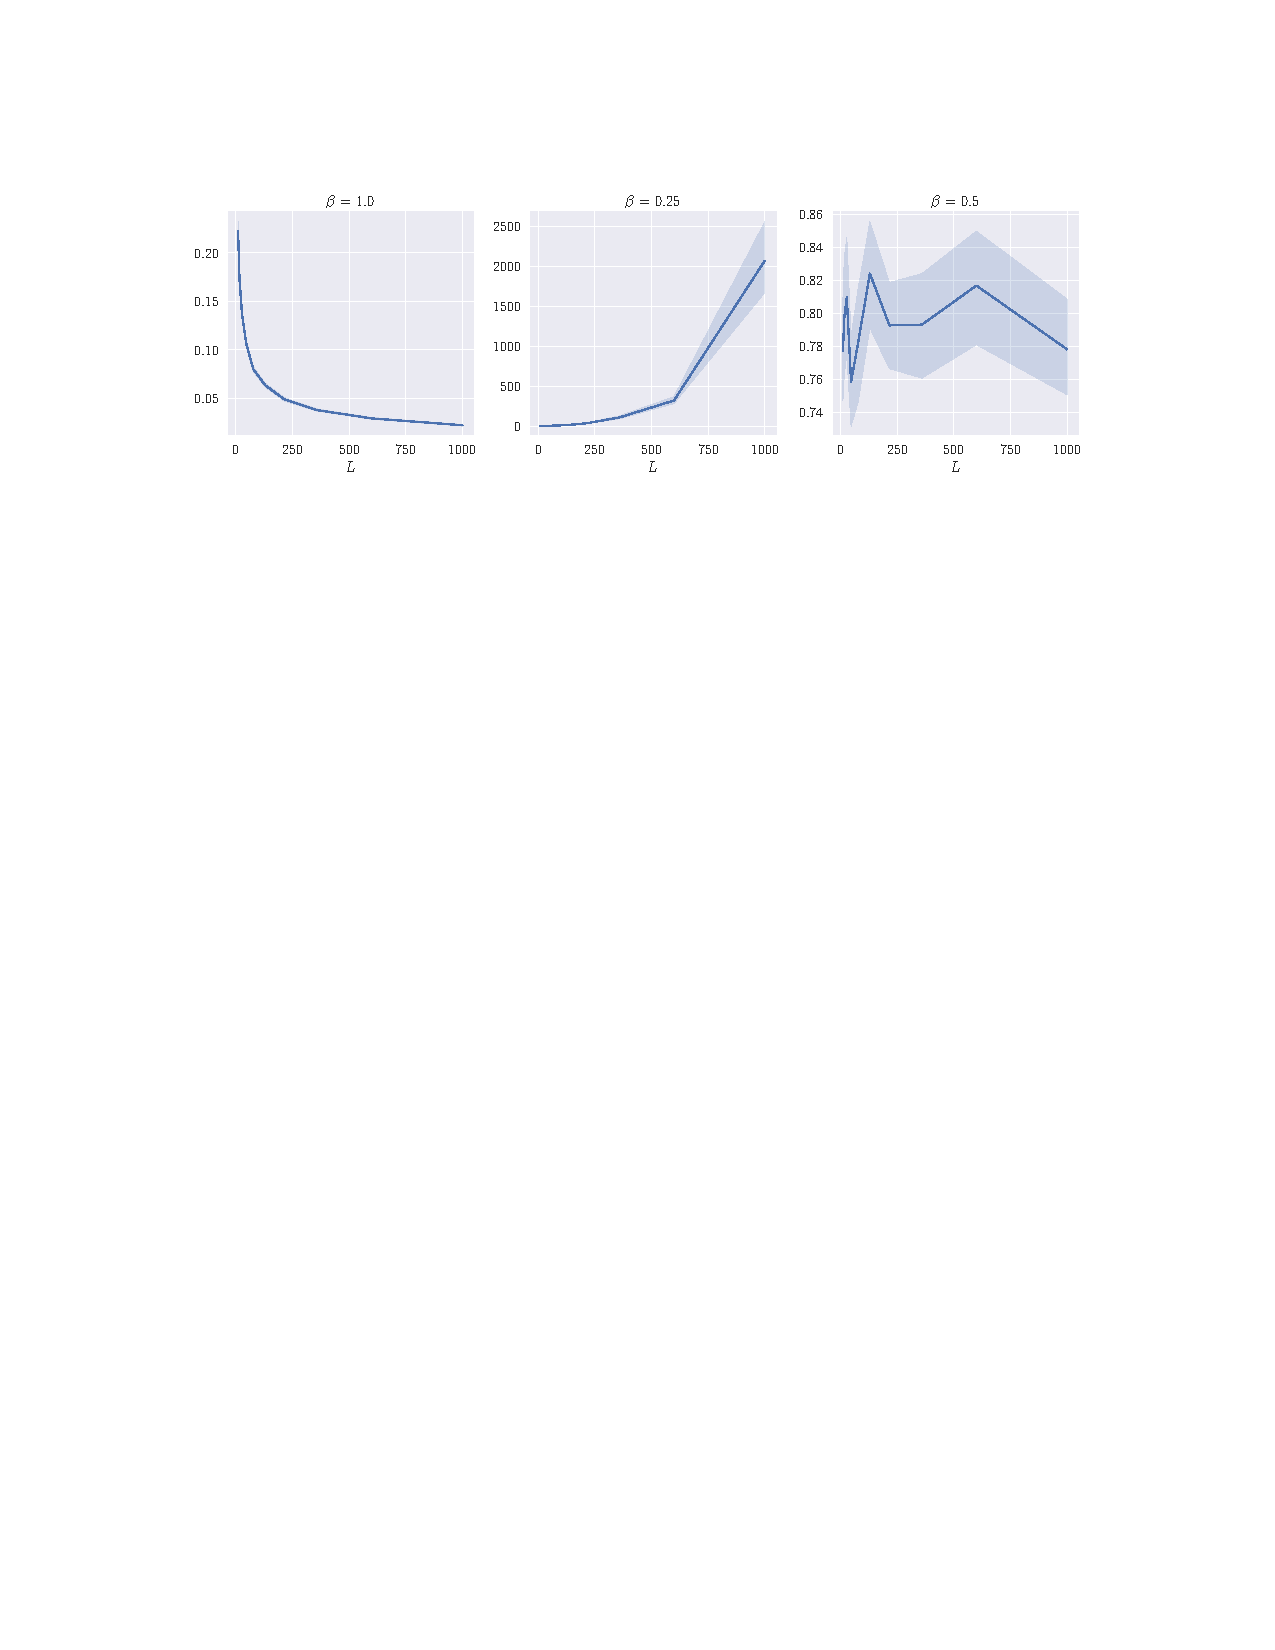
\includegraphics[width=.95\textwidth]{figs/figure_cor4.pdf}
    \caption{Illustration du corollaire \ref{cor4}. Évolution de $ \left\| h_L - h_0 \right\| / \left\| h_0 \right\| $ en fonction de $ L $ pour différente valeur de $ \beta  $.}
    \label{fig:cor4}
\end{figure}


\section{Limite probabilistique des gradients}\label{lim_proba_grad}

Dans la section précédente, nous avons étudié le comportement de la sortie du réseau pour des valeurs élevées de $L$. Cependant, cette analyse ne nous renseigne pas sur le comportement du gradient du coût $p_k = \frac{\partial \mathscr{L}}{\partial h_k} \in \mathbb{R}^d$ durant la rétropropagation, qui est pourtant une donnée cruciale pour évaluer la capacité d'entraînement du réseau à l'initialisation. Par conséquent, cette section se consacrera à l'étude des variations de $\left\| p_0 - p_L \right\| / \left\| p_L \right\|$, toujours dans un contexte où la profondeur du réseau $L$ est grande. Il est important de noter que, en raison de la nature de la rétropropagation, notre attention se porte désormais sur $p_0$ plutôt que sur $p_L$. Nous définissons donc la séquence $(p_k)_{0 \leqslant k \leqslant L}$ comme suit :
\begin{align*}
    \qquad & p_k = p_{k+1} + \alpha _L \frac{\partial g(h_k, \theta _{k+1}) ^T}{\partial h}  V_{k+1}^T p_{k+1} \\
    % \Leftrightarrow & \left\| p_k \right\| ^2 = \left\| p_{k+1} \right\| ^2 + \alpha _L ^2 \left\| \frac{\partial g(h_k, \theta _{k+1}) ^T}{\partial h} V_{k+1}^T p_{k+1} \right\| ^2 + 2 \alpha _L \left\langle p_{k+1}, \frac{\partial g(h_k, \theta _{k+1}) ^T}{\partial h}  V_{k+1}^T p_{k+1} \right\rangle 
\end{align*}
Bien que cette récurrence soit similaire à celle des états cachés (\cref{resnet_equation}), nous ne pouvons pas appliquer les mêmes techniques de preuve utilisées précédement. Cette différence s'explique par la dépendance de $\frac{\partial g(h_k, \theta_{k+1})}{\partial h}$ à $h_k$, et donc à $\theta_1, V_1, \dots, \theta_k, V_k$. Supposer l'indépendance de ces deux quantités serait une hypothèse assez forte, non vérifiée par de nombreuses architectures, comme notre modèle \texttt{res-1}. Ainsi, nous adopterons une autre approche, basée sur la dérivation automatique. Cette méthode nécessite des hypothèses moins contraignantes, mais les résultats obtenus seront exprimés en termes d'espérance plutôt qu'avec une forte probabilité.

Soit $z \in \mathbb{R}^d$. Pour tout $0 \leqslant i, j \leqslant L$, définissons $\frac{\partial h_j}{\partial h_i} \in \mathbb{R}^{d \times d}$ comme la matrice Jacobienne de $h_j$ par rapport à $h_i$. Pour rappel, l'élément en position $(m, n)$ de la Jacobienne représente la dérivée de la $m$-ème coordonnée de $h_j$ par rapport à la $n$-ème coordonnée de $h_i$. Soit $q_k(z) = \frac{\partial h_k}{\partial h_0} z$, en appliquant la règle de la chaîne, nous obtenons
\begin{equation}\label{eq:9}
    q_{k+1}(z) = \frac{\partial h_{k+1}}{\partial h_k} q_k(z) = q_k(z) + \alpha _L V_{k+1} \frac{\partial g(h_k, \theta _{k+1})}{\partial h} q_k(z)
\end{equation}
Nous observons une récurrence similaire à celle présentée dans l'\Cref{resnet_equation}. En considérant maintenant que $z$ est une variable aléatoire suivant une distribution gaussienne, il devient possible de décrire la valeur de $\left\| p_0 \right\| / \left\| p_L \right\|$ en fonction du dernier vecteur $q_L(z)$.
\begin{equation}\label{eq:10}
    \frac{\left\| p_0 \right\| ^2}{\left\| p_L \right\| ^2} = \frac{1}{\left\| p_L \right\| ^2} \mathbb{E}_{z \sim \mathcal{N}(0, I_d)}\left(\left| p_0^T z  \right| ^2 \right) = \mathbb{E}_{z \sim \mathcal{N}(0, I_d)}\left(\left| \left(\frac{p_L}{\left\| p_L \right\| } \right)^T q_L(z) \right| ^2 \right)
\end{equation}
avec $ I_d $ la matrice identité sur $ \mathbb{R}^d $. On retrouve la seconde égalité comme conséquence de 
\[
    p_0^T = \left(\frac{\partial \mathscr{L}}{\partial h_0} \right)^T, z = \left(\frac{\partial \mathscr{L}}{\partial h_0} \right)^T \frac{\partial h_L}{\partial h_0} z = p_L^T  q_L(z)
.\]
En résumé, la récurrence énoncée dans l'équation (\ref{eq:9}) va nous permettre de déterminer les bornes de $\left\| q_L(z) \right\|$. Ces résultats pourront ensuite être transposés à $\left\| p_0 \right\| / \left\| p_L \right\|$ en utilisant l'\Cref{eq:10}. Pour ce faire, il nous faudra établir certaines hypothèses sur le rapport $p_L / \left\| p_L \right\|$.

\subsection*{Hypothèses}

\begin{assumption}\label{H3}
    Soit $ b= p_L / \left\| p_L \right\|  $, alors $ \mathbb{E}(b | h_L) = 0 $ et $ \mathbb{E}(b^T b | h_L) = I_d / d $
\end{assumption}
Cette hypothèse est facilement vérifiée. Par exemple, en considérant $n_{out} = 1$ et en utilisant l'entropie croisée pour une classification binaire, ou bien l'erreur quadratique dans le cadre d'une régression.\\\\
L'hypothèse suivante est l'équivalent pour les gradients de ce qui est énoncé dans \Cref{H2}.
\begin{assumption}\label{H4}
    On a, presque surement, 
    \[
        \frac{\left\| q_k \right\| ^2}{2} \leqslant \mathbb{E}\left(\left\| \frac{\partial g(h_k, \theta _{k+1})}{\partial h} q_k  \right\| ^2 | h_k, q_k \right) \leqslant \left\| q_k \right\| ^2
    .\]
\end{assumption}
L'\Cref{H4} s'applique à toutes les architectures répertoriées dans le \Cref{tab:resnetArchitectures}, comme le démontre la proposition suivante.
\begin{proposition}\label{prop5}
    Soit les réseaux \texttt{res-1}, \texttt{res-2} et \texttt{res-3} définit dans le \Cref{tab:resnetArchitectures}. Supposons l'\Cref{H1} satisfaite et $ \sigma  $ dérivable presque partout avec $ a \leqslant \sigma ^\prime \leqslant b $. Alors
    \begin{itemize}
        \item [(i)] L'\Cref{H4} est valide pour \texttt{res-1}
        \item [(ii)] L'\Cref{H4} est valide pour \texttt{res-2} et \texttt{res-3} dès lors que les entrées de $ \sqrt{d} W_{k+1}, 0 \leqslant k \leqslant L-1 $ sont des variables aléatoires de variance unitaire, i.i.d, symétriques et indépendante de $ d $ et $ L $.
    \end{itemize}
\end{proposition}
Les propositions \Cref{prop6,prop7} sont les homologues des \Cref{prop2,prop3} pour l'analyse du gradient du coût à l'initialisation.
\begin{proposition}\label{prop6}
    Soit un ResNet (\ref{tab:resnetArchitectures}) tel que les \Cref{H1} à \ref{H4} sont satisfaites. Si $ L \alpha _L ^2 \leqslant 1 $ alors, pour tout $ \delta \in (0,1) $ avec une probabilité d'au moins $ 1 - \delta  $ 
    \[
        \frac{\left\| p_0 - p_L \right\| ^2 }{\left\| p_l \right\| ^2 } \leqslant \frac{2 L \alpha _L ^2}{\delta }
    .\]
\end{proposition}

\begin{proposition}\label{prop7}
    Soit un ResNet (\ref{tab:resnetArchitectures}) tel que les \Cref{H1} à \ref{H4} sont satisfaites. Alors 
    \[
        (1 + \frac{1}{2} \alpha _L ^2)^L - 1 \leqslant \mathbb{E}\left( \frac{\left\| p_0 - p_L \right\| ^2 }{\left\| p_l \right\| ^2 } \right) \leqslant (1 + \alpha _L ^2)^L - 1
    .\]
\end{proposition}

De façon similaire au \Cref{cor4}, le \Cref{cor8} est déduit à partir des \Cref{prop6,prop7}.

\begin{cor}\label{cor8}
    Soit un ResNet (\ref{tab:resnetArchitectures}) tel que les Hypothèses 1 à 4 sont satisfaites. En posant $ \alpha _L = 1 / L^\beta $ avec $ B > 0 $, on obtient 
    \begin{enumerate}
        \item [(i)] Si $ \beta > 1/2 $, alors 
        \[
            \frac{\left\| p_0 - p_L \right\| }{\left\| p_l \right\|  } \xrightarrow[L \to \infty]{\mathbb{P}} 0
        .\]
        \item [(ii)] Si $ \beta < 1/2 $ alors 
        \[
            \mathbb{E}\left(\frac{\left\| p_0 - p_L \right\| ^2 }{\left\| p_l \right\| ^2 }\right) \xrightarrow[L \to \infty]{\mathbb{P}} \infty
        .\]
        \item [(iii)] Si $ \beta = 1/2 $ alors
        \[
            \exp \left(\frac{1}{2}\right) - 1 \leqslant \mathbb{E}\left(\frac{\left\| p_0 - p_L \right\| ^2 }{\left\| p_l \right\| ^2 }\right) \leqslant \exp (4) - 1
        .\]
    \end{enumerate}
\end{cor}
Ce corrolaire est illustré dans la \Cref{fig:cor8}. Pour plus d'information sur l'expérience, vous pouvez vous référer au TP.

\begin{figure}[H]
    \centering
    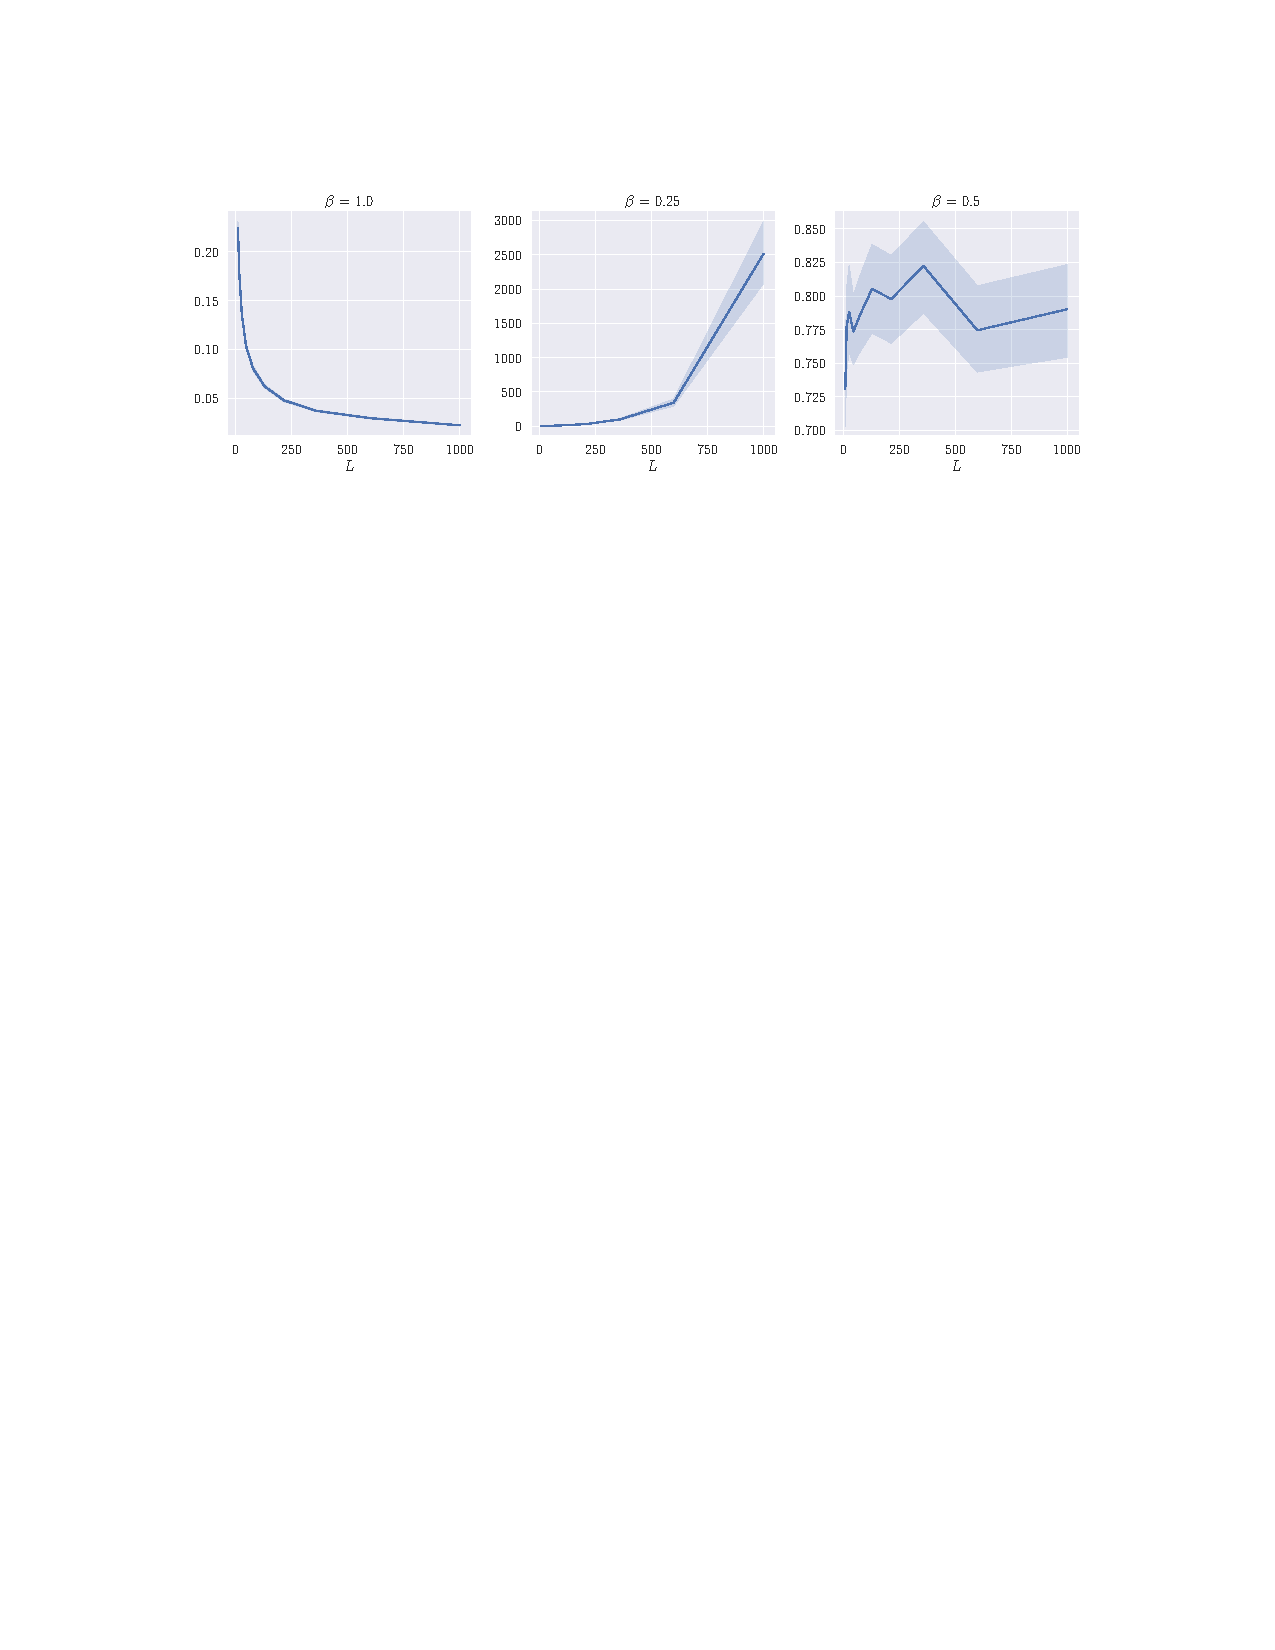
\includegraphics[width=.95\textwidth]{figs/figure_cor8.pdf}
    \caption{Illustration du \Cref{cor8}. Évolution de $ \left\| p_0 - p_L \right\| / \left\| p_L \right\| $ en fonction de $ L $ pour différente valeur de $ \beta  $. Cette figure sera reproduite en TP.}
    \label{fig:cor8}
\end{figure}

\section{Conclusion}\label{ccl_chap2}
Dans ce chapitre, nous avons examiné comment le comportement des gradients et des états cachés est influencé par la valeur de $\beta$, qui se décline en trois cas distincts :
\begin{itemize}
    \item $\beta < 1/2$ : Une explosion qui empêche l'entraînement du réseau.
    \item $\beta > 1/2$ : Un effet d'identité qui diminue les performances du réseau.
    \item $\beta = 1/2$ : Une limite non-dégénérée favorable.
\end{itemize}
Il est intéressant de noter que la valeur $\beta = 1/2$ joue un rôle clé. De manière surprenante, cette valeur trouve une interprétation spécifique dans l'étude des ResNet dans un cadre continu, sujet que nous aborderons dans le chapitre suivant.

\chapter{ODE et SDE}
L’interprétation en temps continu des ResNets fournit un cadre puissant pour comprendre leur comportement, notamment dans le contexte d’architectures d’apprentissage profond comportant un grand nombre de couches.

L’une des principales conclusions est la similarité formelle entre les ResNets mis à l'échelle et les équations différentielles. Comme la profondeur \(L\) tend vers l’infini, le comportement des ResNets peut être approché par un processus continu. Ceci est mathématiquement exprimé comme une transition des mises à jour discrètes par couche dans ResNets vers un système dynamique en temps continu. Plus précisément, l’évolution des états cachés dans un ResNet peut être considérée comme une discrétisation d’une équation différentielle, ce qui constitue une réalisation profonde pour comprendre les modèles d’apprentissage profond.


\section{ODE}
Une ODE est une équation différentielle dans laquelle la fonction inconnue est fonction d'une variable et les dérivées de l'équation impliquent uniquement cette variable. Formellement, ODE peut être exprimé comme $\frac{dy}{dk}=f(k,y)$ où y est fonction de k.
Le but de la résolution d’une équation différentielle du premier ordre est de trouver une fonction y qui satisfait l’équation. Cependant, nous ne pouvons pas calculer directement y
 . Au lieu de cela, nous savons comment la fonction y change avec le temps k, ce qui est représenté par la dérivée $\frac{dy}{dk}$.

 \subsection{ODE neuronale}
 Dans l'apprentissage profond, en particulier lors de la conception de structures de réseau, les équations différentielles ordinaires (ODE) peuvent être utilisées pour décrire les changements dynamiques continus entre les différentes couches du réseau ou les fonctions d'activation.

 La motivation des équations différentielles régulières divines vient de ResNet. ResNet possède généralement une couche non linéaire avec des connexions résiduelles. Nous pouvons résumer cela en une fonction qui représente une fonction non linéaire, une matrice de poids, un biais et une connexion résiduelle.
 \begin{equation}
    h_{k+1} = h_k + f(h_k, \theta_{k+1})
\end{equation}
 En poussant l'espacement entre les couches du réseau à une valeur infinitésimale, nous pouvons convertir ResNet en un réseau neuronal continu, ce qui est exactement ce que fait l'ODE neuronale. En faisant cela, nous pouvons comparer les couches discrètes de ResNet à sa représentation continue de réseau neuronal. Nous pouvons voir que le taux de changement de l’état sous-jacent dans un réseau neuronal continu est déterminé par une fonction non linéaire, et cette fonction ne change pas dans le temps, un peu comme la forme d’une ODE.
 \begin{align*}
 h_{k+1} = h_k + f(h_k, \theta_{k+1}) \\
 \to  h_{k+1} - h_k = f(h_k, \theta_{k+1}) \\
 \to \frac{h_{k+1} - h_k}{1} = f(h_k, \theta_{k+1}) \\
 \to \frac{h_{k+\Delta} - h_k}{\Delta}_{|\Delta=1} = f(h_k, \theta_{k+1}) \\
 \to \lim_{\Delta \to 0} \frac{h_{k+\Delta} - h_k}{\Delta}_{|\Delta=1} = f(h_k, \theta, k) \\
\to \frac{dh(k)}{dt} = f(h_k, \theta, k) \\
\end{align*}

Ici, les couches de réseaux neuronaux traditionnelles sont considérées comme des échantillons discrets d'un système dynamique en temps continu.


 \subsection{Convergence vers une ODE}
 Il est nécessaire de se poser la question de savoir si l'utilisation de méthodes de répartition de poids alternatives lors de l'initialisation et de la mise à l'échelle pourrait conduire à une équation différentielle ordinaire neuronale conventionnelle. Nous supposons que les poids $(V_k)_{1\leqslant k \leqslant L }$ et $(\theta_k)_{1\leqslant k \leqslant L }$ sont des discrétisations de fonctions lisses $\mathcal{V}:[0,1] \to \mathcal{R}^{d*d}$ et $\Theta:[0,1] \to \mathcal{R}^{p}$. On considère alors l’itération générale avant avec $\alpha_L = \frac{1}{L}$, soit:
 \begin{equation}
     h_0 = Ax,\ h_{k+1} = h_k + \frac{1}{L}V_{k+1}g(h_k,\theta_{k+1}),\ 0 \leqslant k \leqslant L-1
 \end{equation}
avec $V_k = \mathcal{V}_{k/L}$ et $\theta_k = \Theta_{k/L}$.
Combiner avec l'idée de Neural ODE avant, on considère $(V_k)_{1\leqslant k \leqslant L }$ et $(\theta_k)_{1\leqslant k \leqslant L }$ sont variables aléatoires en mettant $(\mathcal{V}_t)_{t \in [0,1]}$ et $(\Theta_t)_{t \in [0,1]}$ sont les temps continus
processus stochastiques. Dans ce modèle, nous aurons besoin de les hypothèses suivantes. Ces hypothèses constituent la base d'une dérivation théorique ultérieure et garantissent que les outils et méthodes mathématiques utilisés sont adaptés à l'analyse des modèles neuronale. 

\begin{assumption}\label{H5}
Pour chaque $0 \leqslant k \leqslant L-1$, les processus stochastique $\mathcal{V}$ et $\Theta$ sont presque sûrement Lipschitziens continus et bornés.
\end{assumption}

Plus précisément, il existe presque sûrement $K_{\mathscr{V}}, K_{\Theta}, C_{\mathscr{V}}, C_{\Theta}>0,tel que, pour tous s, t \in[0,1]$

$$
\left\|\mathscr{V}_t-\mathscr{V}_s\right\| \leqslant K_{\mathscr{V}}|t-s|, \quad\left\|\Theta_t-\Theta_s\right\| \leqslant K_{\Theta}|t-s|, \quad\left\|\mathscr{V}_t\right\| \leqslant C_{\mathscr{V}}, \quad\left\|\Theta_t\right\| \leqslant C_{\Theta} .
$$

\begin{assumption}\label{H6}
 La fonction g est Lipschitzienne continue sur les ensembles compacts, dans le sens où pour tout compact $\mathscr{P} \subseteq \mathbb{R}^p$, il existe $K_{\mathscr{P}} > 0$  tel que, pour tous $h, h^{\prime} \in \mathbb{R}^d, \theta \in \mathscr{P}$,
$$
\left\|g(h, \theta)-g\left(h^{\prime}, \theta\right)\right\| \leqslant K_{\mathscr{P}}\left\|h-h^{\prime}\right\|,
$$
et pour tous compact $\mathscr{D} \subseteq \mathbb{R}^d$, il existe $K_{\mathscr{D}, \mathscr{P}}>0$ tel que, pour tous $h \in \mathscr{D}, \theta, \theta^{\prime} \in \mathscr{P}$,
$$
\left\|g(h, \theta)-g\left(h, \theta^{\prime}\right)\right\| \leqslant K_{\mathscr{D}, \mathscr{P}}\left\|\theta-\theta^{\prime}\right\| .
$$
\end{assumption}


Sous les hypothèses \ref{H5} et \ref{H6}, la récurrence (2.2) converge presque sûrement vers l'ODE neuronale donnée par
$$
H_0=A x, \quad d H_t=\mathscr{V}_t g\left(H_t, \Theta_t\right) d t, \quad t \in[0,1]
$$
comme la proposition ci-dessous.

\begin{proposition}\label
Considérons le modèle (2.2) tel que les hypothèses \ref{H5} et \ref{H6} sont satisfaites. Alors l'ODE (2.3) a une solution unique H, et, presque sûrement, il existe un $c > 0$
tel que, pour tout $0 \leqslant k \leqslant L$,

\begin{equation}  
\left\|H_{k / L}-h_k\right\| \leqslant \frac{c}{L}
\end{equation}
\end{proposition}

En supposant que les poids du réseau sont des discrétisations d'une fonction lisse (hypothèse \ref{H5}), il est possible d'obtenir des résultats de stabilité, en fonction de la valeur de $\beta$.

Nous montrons ci-dessous que $\beta$ est une valeur critique, en examinant les états cachés. Nous avons la proposition suivant.

\begin{proposition}
    Sous les hypothèses \ref{H5} et \ref{H6}, on fait $\alpha_L = \frac{1}{L^{\beta}}$, avec $\beta >0 $.
    \item si $\beta > 1 $, alors presque sûrement, $\lim_{L \to \infty}\frac{||h_L-h_0||}{h_0} = 0 $
    \item si $\beta = 1 $ ,alors presque sûrement,il existe un c > 0 tel que $\frac{||h_L-h_0||}{h_0} \leqslant c$
    \item si $\beta < 1 $, Le cas de l'explosion est plus délicat à traiter, on ne disscute pas ici.
\end{proposition}

\begin{proof}\label{prop 4}
En utilisant hypothèse \ref{H6},on peux facilement obtenir l'existence de $C_1$ et $C_2$ (ses valeurs depend en de réalisation de $\mathscr{V}$ and $\Theta$ ) tel que
$$
\left\|h_{k+1}\right\| \leqslant\left(1+C_1 \alpha_L\right)\left\|h_k\right\|+C_2 \alpha_L
$$

Par récurrence,
$$
\left\|h_{k+1}\right\| \leqslant\left(1+C_1 \alpha_L\right)^k\left(\left\|h_0\right\|+\frac{C_2}{C_1}\right) .
$$


Puis, utiliser $\alpha_L \leqslant 1 / L$,
$$
\left\|h_{k+1}\right\| \leqslant \exp \left(C_1\right)\left(\left\|h_0\right\|+\frac{C_2}{C_1}\right) .
$$

Car $g$ est lipschitzien continu en ensemble compact, il est délimité sur chaque boule de $\mathbb{R}^d \times \mathbb{R}^p$. Le résultat est alors une conséquence de l’identité
$$
h_L-h_0=\alpha_L \sum_{k=0}^{L-1} V_{k+1} g\left(h_k, \theta_{k+1}\right)
$$
puisque nous avons montré que chaque terme de la somme est borné par une constante $C_3>0$, indépendante de $L$ et $k$. Nous avons donc cela 
$$
\left\|h_L-h_0\right\| \leqslant C_3 L \alpha_L=C_3 L^{1-\beta},
$$
donnant les résultats en fonction de la valeur de $\beta$.
\end{proof}

\begin{proposition}\label
    On considère la modèle "res-1": $h_{k+1} = h_k +\alpha_{L}V_{k+1}\sigma(h_k) $ ,en prenant $\sigma$ comme fonction d'identité. Supposons que l'hypothèse \ref{H5} soit satisfaite et que $\mathcal{V_0^{T}}$ ait une valeur propre positive. $\alpha_L = \frac{1}{L^{\beta}}$,avec $\beta \in (0,1)$. Alors, $\max_{k}\frac{||h_k-h_0||}{||h_0||} \to \infty$ quand $L \to \infty$
\end{proposition}

Dans ce contexte, nous pouvons observer expérimentalement une évolution du comportement de la sortie et des gradients lorsque la valeur de L augmente, similaire à celle explorée dans la section précédente.  Cependant, le point remarquable est que la séparation se produit pour $\beta = 1$ ici.

\section{SDE}
SDE est une extension de ODE, qui contient un terme aléatoire et est généralement utilisée pour simuler l'influence de processus aléatoires ou de bruit. Formellement, SDE peut être exprimé comme $dy = f(k,y)dk + g(k,y)dW $, W signifie mouvement brownien ou processus de Wiener. 
SDE est utilisé en apprentissage profond pour simuler des systèmes contenant du caractère aléatoire, tels que le bruit lors de l'entraînement, l'initialisation aléatoire des poids, etc. Cela permet de comprendre et d'analyser le comportement des réseaux face à des perturbations aléatoires.

\subsection{SDE neuronale}
Par rapport à Neural ODE, Neural SDE introduit le caractère aléatoire, ce qui permet au modèle de mieux gérer l'incertitude et le bruit des données.
On prends W comme le mouvement brownien ici.

Le mouvement brownien est un modèle mathématique utilisé pour décrire le chemin d'une marche aléatoire. En apprentissage profond, il peut être utilisé pour simuler des fluctuations aléatoires dans les mises à jour de poids ou les valeurs d'activation, en particulier dans les réseaux profonds, où ces fluctuations peuvent s'accumuler à mesure que le nombre de couches augmente.

\begin{definition}\label
Le mouvement brownien unidimensionnel $(B_t)_{t \geq 0} $ est un processus stochastique continu,avec des incréments indépendants, dépendant du temps t et vérifiant : $B_0 = 0$ et pour tous $0 \leq s \le t \leq 1, B_t - B_s \sim \mathcal{N}(0,t-s)$.
\end{definition}

L'un des principaux messages de la section 2 est que l'initialisation standard avec les paramètres i.i.d. conduit à un modèle non dégénéré pour les grandes valeurs de L seul en 
$L\alpha_L^2 \approx 1$. Or pour $\beta = 1/2$ quand $\alpha_L=\frac{1}{L^{\beta}}$ 

(Par les propositions et corollaires d'avance). De manière remarquable, il convient de noter que ce régime correspond à la discrétisation d'un SDE dans la limite du temps continu. Pour étayer cette affirmation, prenons en compte, à des fins de simplification, le modèle ResNet res-1, qui est discret.
\begin{equation}
    h_{k+1} = h_k + \frac{1}{\sqrt{L}}V_{k+1}\sigma(h_k) , 0 \leq k \leq L-1 
\end{equation}

où les entrées de $V_{k+1}$ sont supposées être i.i.d $\mathcal{N}(0,2/d)$.
Maintenant, on pass $\mathbf{B}:[0,1] \rightarrow \mathbb{R}^{d \times d}$ comme un$(d \times d)$-dimension movement brownie, dans le sens où le $\left(B_{i j}\right)_{1 \leqslant i, j \leqslant d}$ sont unidimensionnel mouvement brownien. Donc, pour tous $0 \leqslant k \leqslant L-1$ et tous $1 \leqslant i, j \leqslant d$, on a
$$
\mathbf{B}_{(k+1) / L, i, j}-\mathbf{B}_{k / L, i, j} \sim \mathcal{N}\left(0, \frac{1}{L}\right),
$$
et les incréments pour différentes valeurs de $(i, j, k)$ sont indépendants. En conséquence, la récurrence (2.4) est équivalente en distribution à la récurrence
$$
h_{k+1}^{\top}=h_k^{\top}+\sqrt{\frac{2}{d}} \sigma\left(h_k^{\top}\right)\left(\mathbf{B}_{(k+1) / L}-\mathbf{B}_{k / L}\right), \quad 0 \leqslant k \leqslant L-1 .
$$
($V_{k+1}$ a meme distribution de $V_{k+1}^{\top}$.) On peut obtenir que $\{k / L, 0 \leqslant k \leqslant L\}$ 
\begin{equation}
    d H_t^{\top}=\sqrt{\frac{2}{d}} \sigma\left(H_t^{\top}\right) d \mathbf{B}_t, \quad t \in[0,1]
\end{equation}
où la sortie du réseau est désormais fonction de la valeur finale de H, c'est-à-dire H1. Le
Le lien entre le ResNet discret (2.4) et le SDE (2.5) est formalisé dans la proposition suivante.

\begin{proposition}\label
 Considérons le modèle res-1, où les entrées de $V_{k+1}$ sont i.i.d. Variables aléatoires gaussiennes $\mathcal{N}(0,2 / d)$. Supposons que la fonction d'activation $\sigma$ soit continue de Lipschitz. Alors le SDE (2.5) a une unique solution $H$ et, pour tout $0 \leqslant k \leqslant L$,
$$
\mathbb{E}\left(\left\|H_{k / L}-h_k\right\|\right) \leqslant \frac{c}{\sqrt{L}}
$$
for some $c>0$.
\end{proposition}

\begin{proof}\label
    La proposition est une conséquence de Kloeden et Platen (1992, théorèmes 4.5.3 et 10.2.2) pour le SDE
$$
d H_t^{\top}=\sqrt{\frac{d}{2}} \sigma\left(H_t^{\top}\right) d B_t
$$

Supposons $a(h, t)=0$ et $b(h, t)=\sqrt{\frac{d}{2}} \sigma(h)$,On doit verifier les hypos suivants:

$\left(H_1\right)$ Les fonctions $a(\cdot, \cdot)$ et $b(\cdot, \cdot)$ sont jointe mesurables en $\mathbb{R}^d \times[0,1]$.


$\left(H_2\right)$ Il existe un constante  $C_1>0$ tel que, pour tous $x, y \in \mathbb{R}^d, t \in[0,1]$,
$$
\|a(x, t)-a(y, t)\|+\|b(x, t)-b(y, t)\| \leqslant C_1\|x-y\| .
$$

$\left(H_3\right)$ Il existe un constante $C_2>0$ tel que, pour tous $x \in \mathbb{R}^d, t \in[0,1]$,
$$
\|a(x, t)\|+\|b(x, t)\| \leqslant C_2(1+\|x\|) .
$$

$\left(H_4\right) \mathbb{E}\left(\mid H_0 \|^2\right)<\infty$.

$\left(H_5\right)$ Il existe un constante $C_3>0$ tel que, pour tous $x \in \mathbb{R}^d, s, t \in[0,1]$,
$$
\|a(x, t)-a(x, s)\|+\|b(x, t)-b(x, s)\| \leqslant C_3(1+\|x\|)|t-s|^{1 / 2} .
$$

Hypos $\left(H_1\right),\left(H_4\right)$, et $\left(H_5\right)$ découlent facilement des définitions.
Hypo $\left(H_2\right)$ est vrai puisque $\sigma$ est lipschitz continu et $\left(H_3\right)$ découle de
$$
\|\sigma(x)\| \leqslant b\|x\| \leqslant\|x\| \leqslant 1+\|x\| .
$$
\end{proof}

Lorsque le facteur d'échelle $\bets$ est fixé à 1/2, cela produit non seulement une dynamique non triviale à l'initialisation, mais correspond également à un modèle de diffusion simple dans le modèle en temps continu. Ce point montre que les réseaux de neurones très profonds sont en fait équivalents à la solution de SDE lors de l’utilisation d’une initialisation de poids indépendante et identiquement distribuée (i.i.d.).

\section{Conclusion}
La plupart des fonctions d'activation classiques (telles que ReLU) satisfont à l'exigence continue de Lipschitz. Cela indique que ces fonctions ont certaines limites en termes de taux de changement, ce qui est important pour la stabilité et la prévisibilité du réseau.

\begin{enumerate}
    \item Lorsque le facteur d'échelle $\beta$ = 1 ($\alpha$ = $\frac{1}{L}$)et que l'initialisation des poids n'est pas i.i.d., le modèle correspondant tend à ODE.
    Parce que les poids ne sont pas identifiés, le comportement du réseau est plus déterministe et peut être affecté par une stratégie d'initialisation ou une distribution de poids spécifique. Dans ce cas, il est approprié d'utiliser des ODE pour simuler le comportement du réseau, car les ODE fournissent un moyen d'analyser les systèmes dynamiques dans un cadre déterministe.

    \item Lorsque le facteur d'échelle $\beta$ = 1/2 ($\alpha$ = $\frac{1}{\sqrt{L}}$) et que l'initialisation des poids est i.i.d., le modèle correspondant tend à SDE.
\end{enumerate}

Dans l'ensemble, le choix d'utiliser SDE ou ODE dépend de la nature des poids dans le modèle (iid ou non-iid) et du comportement du réseau que nous souhaitons capturer (stochastique ou déterministe).

Ce modèle est intéressant dans la mesure où le mouvement brownien (SDE) est ($\frac{1}{2}-\epsilon$)-Holder, un processus stochastique continu lipschitz (ODE) est 1-Holder.

Il est important de noter que le choix de la mise à l'échelle d'un ResNet semble être étroitement lié à la régularité des poids en fonction de la couche. Plus précisément, dans tous les régimes, le facteur d'échelle critique entre l'explosion et l'identité semble être étroitement lié à la régularité des poids en fonction de la couche. Ces résultats ont une interprétation naturelle en termes de régularité (Holder) du processus stochastique en temps continu sous-jacent.

Ces modèles en temps continu, à la fois équations différentielles ordinaires (ODE) et équations différentielles stochastiques (SDE), offrent un cadre exhaustif pour l'analyse et l'interprétation du comportement des réseaux de neurones résiduels (ResNets) profonds. Ils établissent ainsi un lien entre les architectures de deep learning discrètes et la théorie approfondie des équations différentielles.

\chapter{Conclusion}
Ce tutoriel présente une analyse complète des défis liés à la mise à l'échelle dans les ResNets profonds. Il met en évidence l'importance du facteur de mise à l'échelle \(\alpha_L\), de l'analyse probabiliste et des informations fournies par les modèles en temps continu. En combinant une analyse théorique et des preuves empiriques, on parvient à une compréhension approfondie des mécanismes impliqués dans la formation des ResNets profonds. Cette approche ouvre la voie à la création d'architectures d'apprentissage profond plus efficaces et efficientes à l'avenir.

Premièrement, il convient de mentionner que les Resnets ont été un véritable exploit dans le domaine de l'apprentissage automatique complexe. Ils ont été les premiers modèles de réseaux neuronaux profonds à être entraînés avec succès avec un grand nombre de couches, ce qui a considérablement amélioré les performances. Étant donné son application étendue et son importance, il est essentiel de réfléchir à la manière de construire un cadre "parfait" afin d'éviter tout problème de disparition ou d'explosion de gradient lors de l'entraînement en profondeur, qui pourrait conduire à de mauvais résultats.

Deuxièmement, nous avons constaté, à travers de nombreuses expériences, que la répartition des valeurs initiales (les poids $(V_k)_{1\leqslant k \leqslant L }$ et $(\theta_k)_{1\leqslant k \leqslant L }$)joue un rôle crucial dans les résultats de l'entraînement. Par conséquent, il est impératif d'examiner attentivement la régularité de l'évolution des poids dans le processus de descente de gradient et son impact sur la dynamique de l'entraînement.

La relation entre le taux d'apprentissage et le facteur de mise à l'échelle $\alpha_{L}$ joue un rôle essentiel dans l'évaluation plus précise de la corrélation entre les performances du réseau formé et la mise à l'échelle.

\bibliographystyle{plainnat} % We choose the "plain" reference style
\bibliography{bib} % Entries are in the refs.bib file

\end{document}